
\section{Globular Clusters}


Globular clusters (GCs) are dense, spheroidal collections of hundreds of thousands of stars bound by
their own self-gravity. GCs are found in most galaxies, with the Milky Way hosting roughly 150,
mostly located in the outer halo \citep{Heggie2003}. GCs represent some of the oldest stellar
populations in the universe and are usually in excess of 10 billion years old. Figure
\ref{fig:1/ngc7006} shows the globular cluster NGC\,7006, imaged by the Hubble Space Telescope's
Advanced Camera for Surveys. The dense core of the cluster is clearly visible and is made up of tens
of thousands of stars. The dynamics of globular clusters are almost entirely governed by the
interactions between individual cluster members, with small effects from the galactic potential of
its host galaxy as well as mass loss due to stellar evolution. Two-body relaxation is essentially
the main driver of the evolution of GCs and through this process, they display a wide range of dynamical
phenomena. Among these phenomena, mass segregation is a process through which heavier objects
migrate to the centre of a cluster and lighter objects move to the outer regions. As objects
interact with each other, their kinetic energies will tend to equalize which leads to heavier
objects slowing down and lighter objects speeding up \citep{Heggie2003}. This process leads to the
core of the cluster containing a much higher proportion of high-mass stars and heavy remnants than
the rest of the cluster. Figure \ref{fig:1/radial_mean_mass} shows the mean mass of objects within a
realistic model of a globular cluster as a function of distance from the cluster centre. The regions
closest to the core of the cluster have a much higher mean mass due to the increased presence of
heavy remnants and high-mass stars caused by the effects of mass segregation.

\begin{figure}
	\centering
	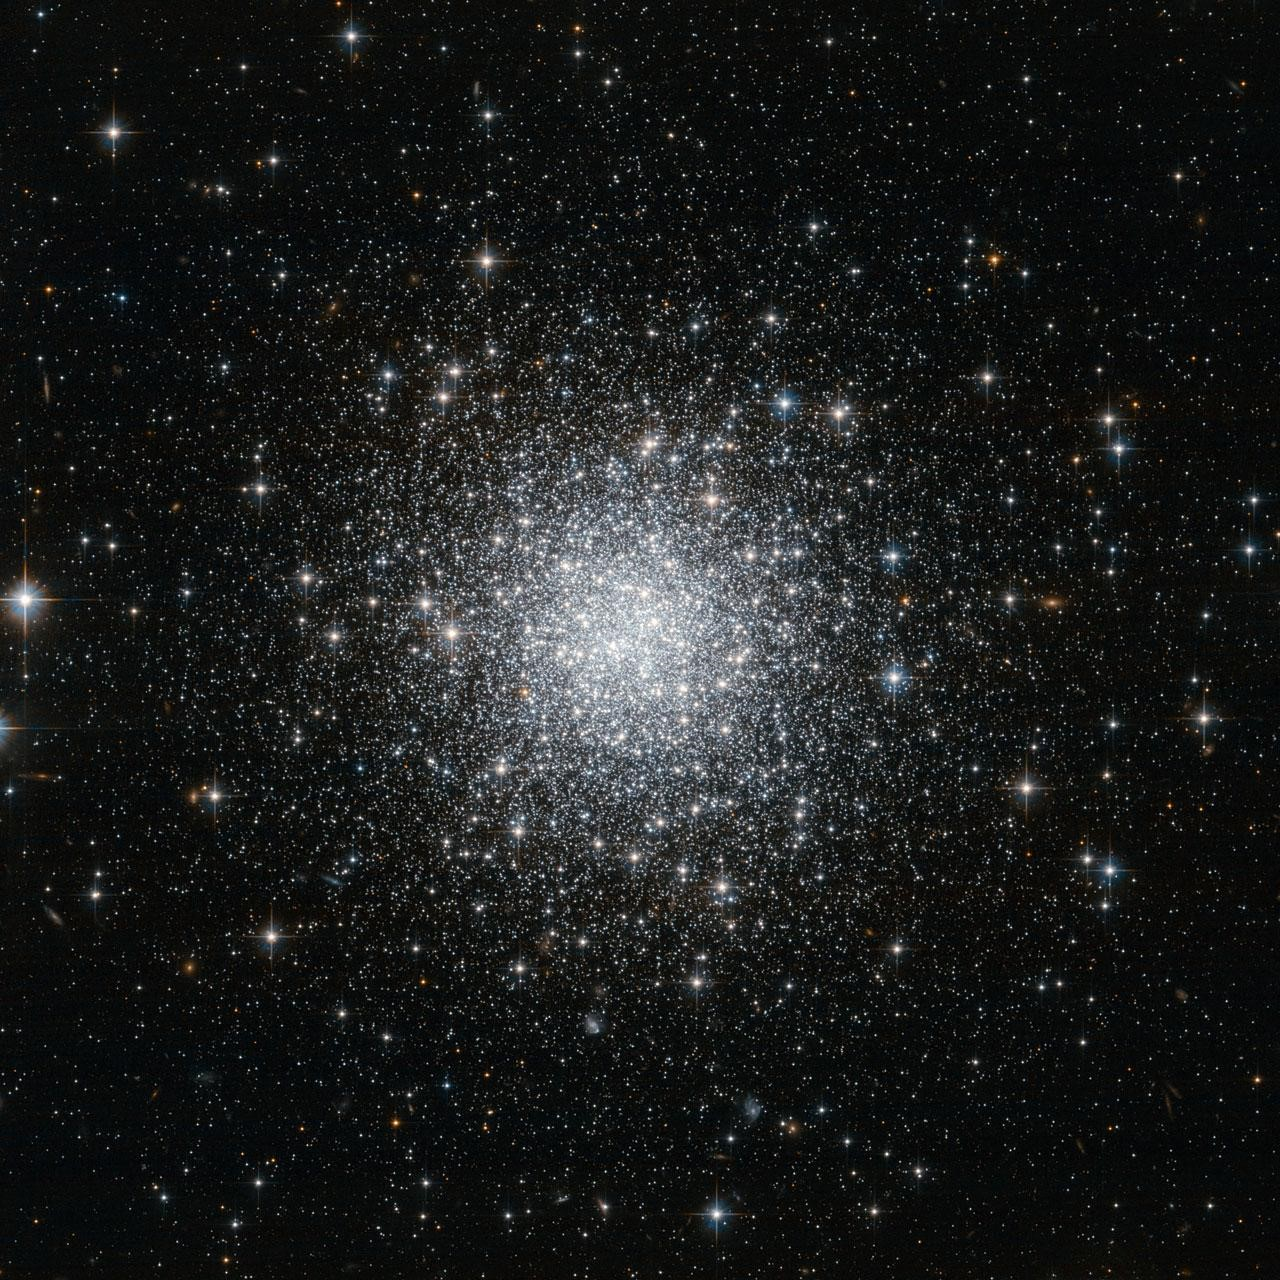
\includegraphics[width=0.8\textwidth]{figures/c42.jpg}
	\caption{The globular cluster NGC 7006 imaged by the Hubble Space Telescope's Advanced
		Camera for Surveys, photo courtesy of ESA/Hubble \& NASA}
	\label{fig:1/ngc7006}
\end{figure}



The study of stellar remnants in globular clusters has far-reaching implications for diverse fields
of astrophysics. Globular clusters are one of the most commonly proposed candidates to host
intermediate-mass black holes (IMBHs). Due to the effects of mass segregation and the high densities
within the cores of globular clusters, the central regions of globular clusters are an ideal
environment for mergers of compact objects \citep{Rodriguez2021}. These mergers can be detected
through their resultant gravitational waves and the expected rates for gravitational wave events
depend significantly on the compact object populations in globular clusters. These mergers are also
thought to be one of the most promising formation channels for IMBHs \citep{Giersz2015}, a so-far
undetected class of black holes whose masses fall between those of stellar-mass black holes and
those of supermassive black holes. The formation of these black holes has important implications for
understanding the formation of the supermassive black holes that we find at the centre of galaxies.


The work presented in this thesis builds on a previous project I worked on which used pulsar timing
data to constrain the properties of the globular cluster 47\,Tuc. In that work, we were able to
place strong limits on the mass in dark remnants (black holes, neutron stars, white dwarfs) within
the cluster, establishing strong constraints on the black hole content specifically. While this
project was able to fully account for effects like mass segregation and uncertain mass functions,
one limitation of the models that it used (which we will discuss in the following section) was the
assumption that all objects within the cluster are single. Because the masses of some binary stars
are higher than the typical masses of objects within the cluster, they too will mass segregate to
the core of the cluster like heavy stellar remnants. While the binary fraction in 47\,Tuc is
expected to be quite low \citep{Milone2012}, the effects that a centrally concentrated population of
binary stars might have on the inferred remnant content of the cluster is still unclear and worth
investigating.



\begin{figure}
	\centering
	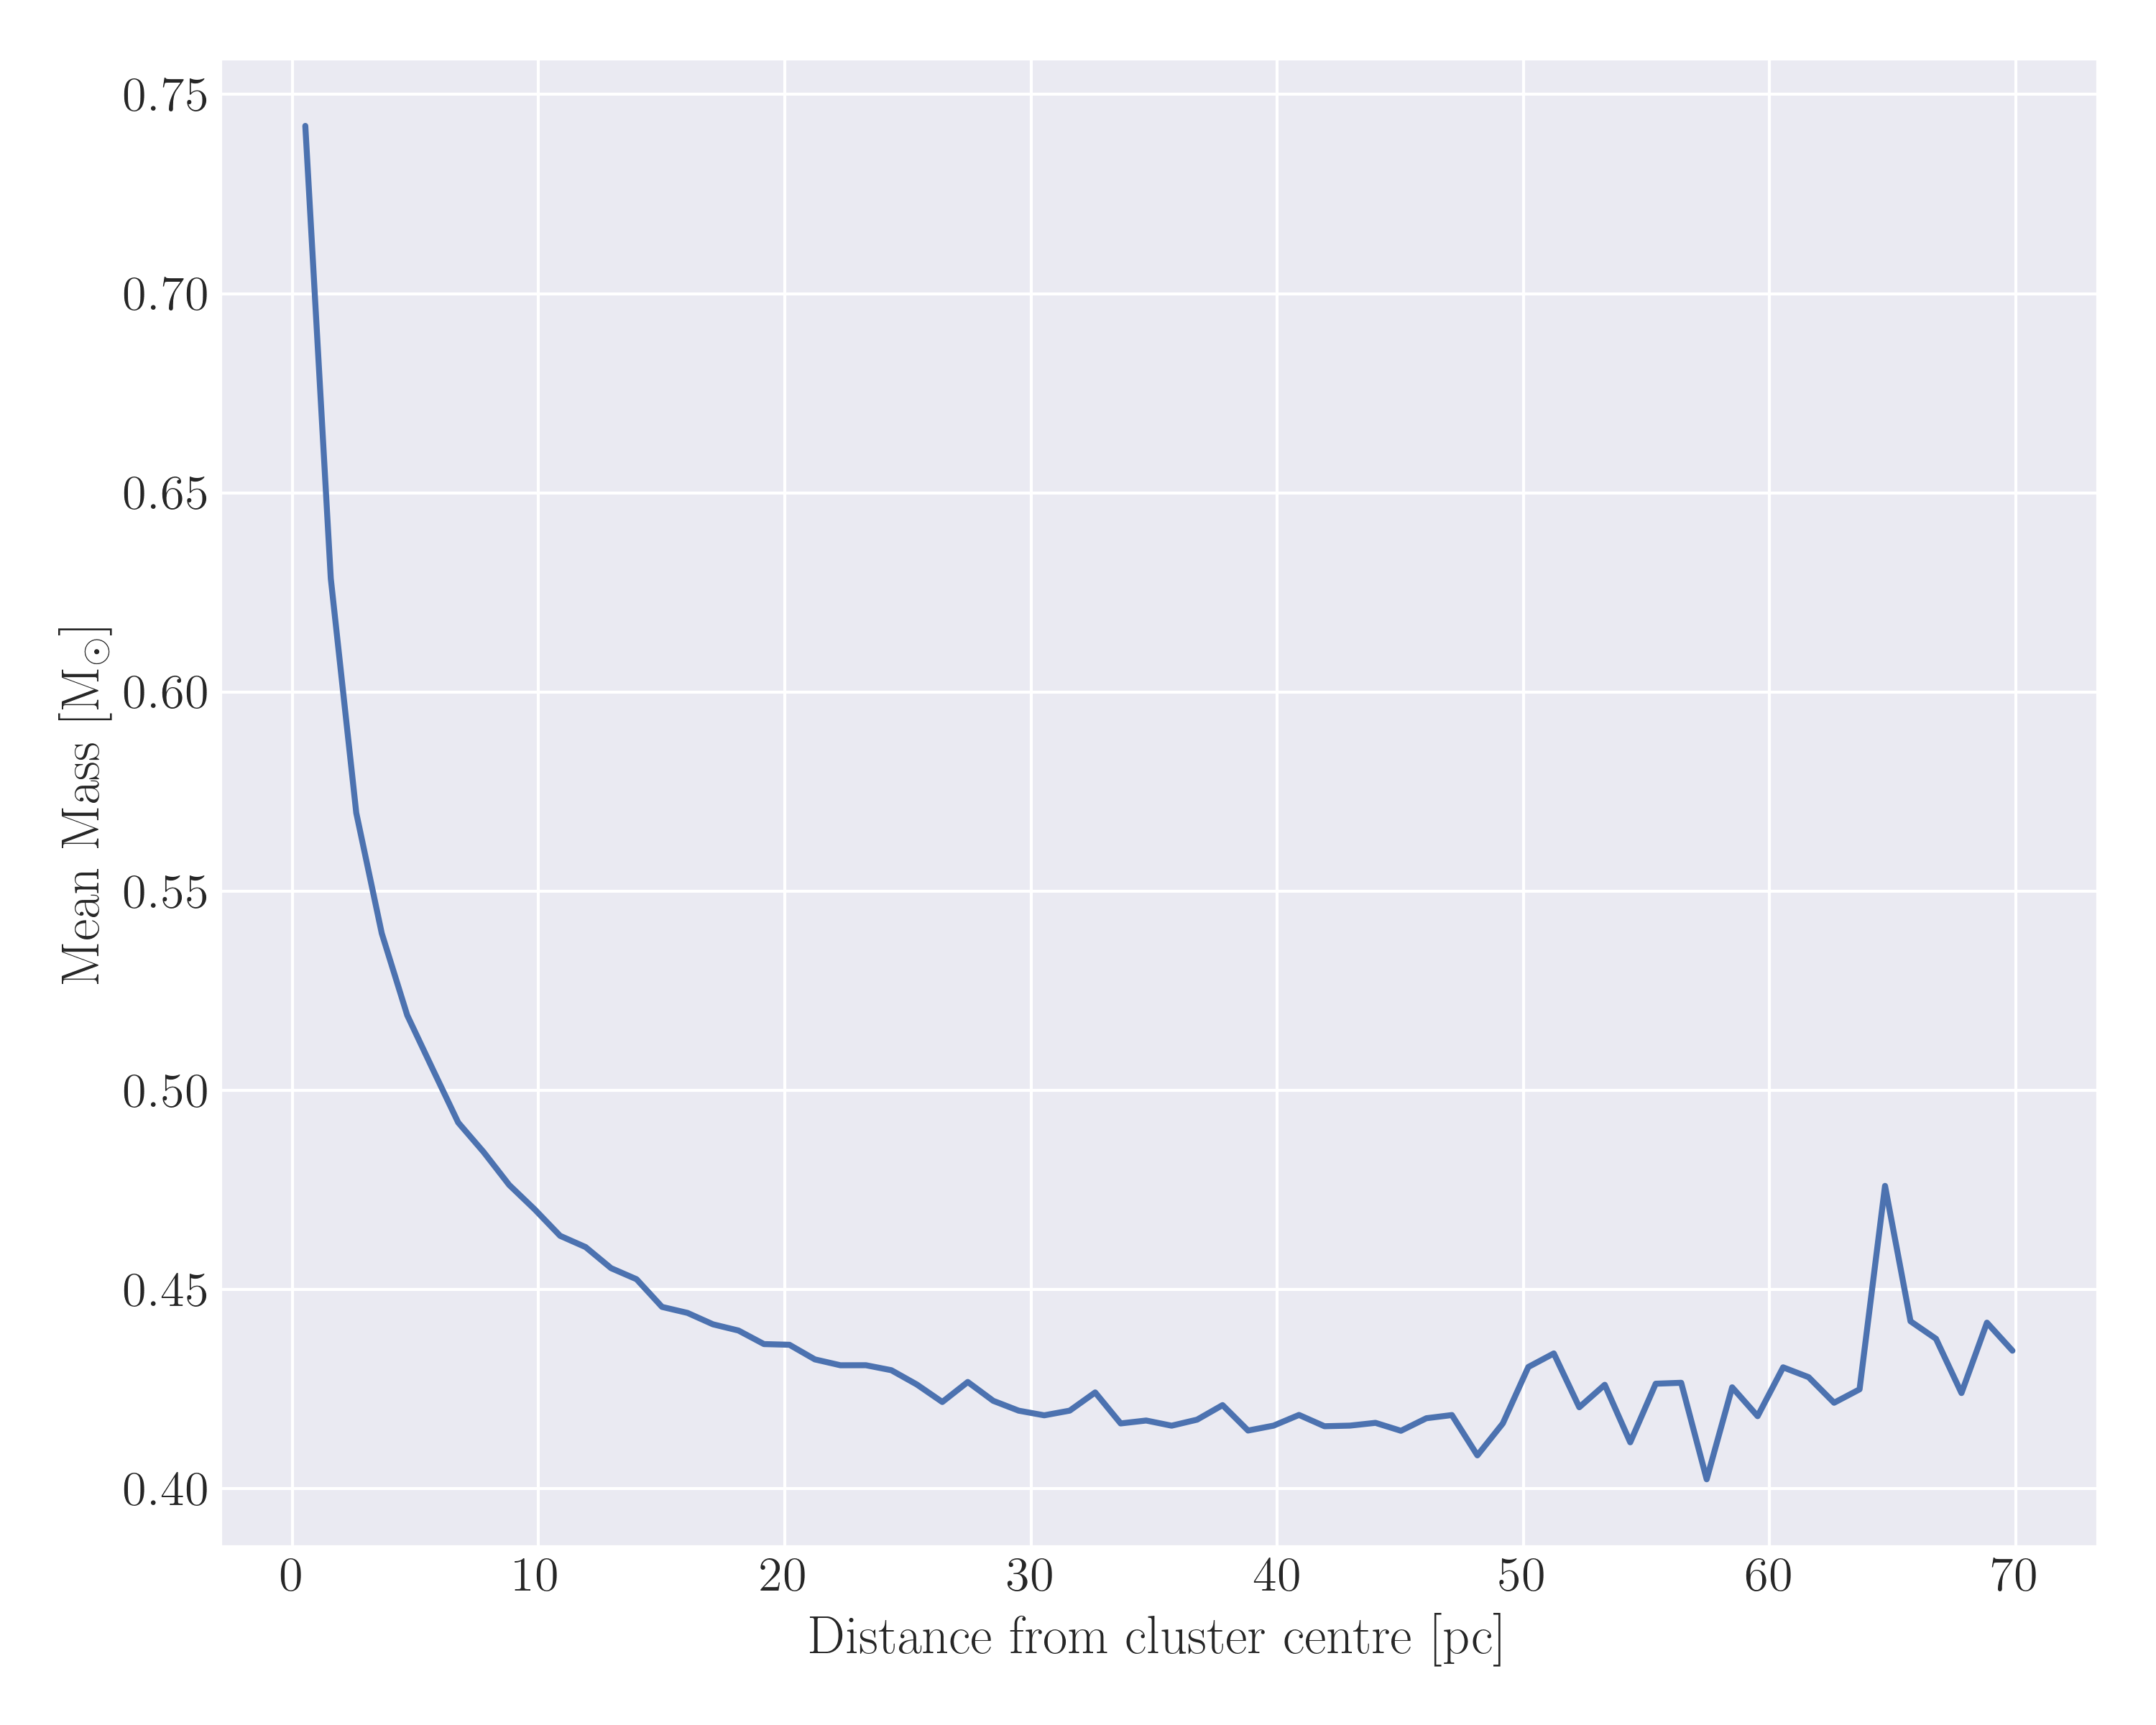
\includegraphics[width=0.8\textwidth]{figures/radial_mean_mass.png}
	\caption{Mean mass of objects within a realistic model of the globular cluster 47\,Tuc, as a
function of distance from the cluster centre. The concentration of high-mass objects
in the central regions of the cluster is obvious, as is the preference for low-mass
objects in the outskirts of the cluster, clearly demonstrating the effects of mass
segregation.}
	\label{fig:1/radial_mean_mass}
\end{figure}




\section{Modelling Globular Clusters}

\paragraph{}


When modelling the dynamics of globular clusters, there are generally two approaches commonly used.
The first is to model the entire evolutionary history of the cluster from initial conditions to the
present day. The most commonly employed versions of these "evolutionary models" are direct N-body
integration (see for example \citealt{Baumgardt2017a}) which directly calculate the gravitational
interactions between each object in the cluster and Monte Carlo models (e.g.
\citealt{Rodriguez2021}, \citealt{Hypki2013}) which approximate the gravitational interactions
between objects according to the method of \citet{Henon1971}. While these models provide insight
into the dynamical history of the cluster, they are very computationally expensive with even the
fastest models taking on the order of a day to model a realistic globular cluster
\citep{Rodriguez2021}.

The second approach is to model just the present-day conditions of the cluster. These models, which
we call "equilibrium models", capture none of the dynamical history of the cluster but fully
describe the present-day state of the cluster. These equilibrium models are much less
computationally demanding than evolutionary models. Their relative efficiency allows us to explore a
significantly larger parameter space when fitting the models to observations to constrain the
present-day properties of a cluster. In particular, it is worth highlighting that by using
equilibrium models, we are able to vary the stellar mass function of the cluster as well as the
black hole and remnant retention fractions with more flexibility than what might be possible with
evolutionary models, due to the computational cost of computing extensive grids of evolutionary
models with many parameters varied in the initial conditions (e.g. various stellar initial mass
functions, initial cluster radii, masses, etc.).

The comparative efficiency of these models further enables the use of statistical fitting techniques
like MCMC or Nested Sampling which would be prohibitively expensive to use with evolutionary models.
This means that instead of computing a grid of models and finding the "best-fitting" model we can
instead recover posterior distributions for key cluster parameters.


In this work, we use the \code{LIMEPY} family of models presented by \citet{Gieles2015}. The
\code{LIMEPY} models are a set of distribution function-based equilibrium models that are isothermal
for the most bound stars near the cluster centre and described by polytropes in the outer regions
near the escape energy. The models have been extensively tested against $N$-body models
\citep{Zocchi2016, Peuten2017} and are able to effectively reproduce the effects of mass
segregation. Their suitability for mass modelling globular clusters has been tested on mock data
\citep{Henault-Brunet2019} and they have recently been applied to real datasets as well
\citep[e.g.][]{Gieles2018, Henault-Brunet2020}.


\begin{figure}
	\centering
	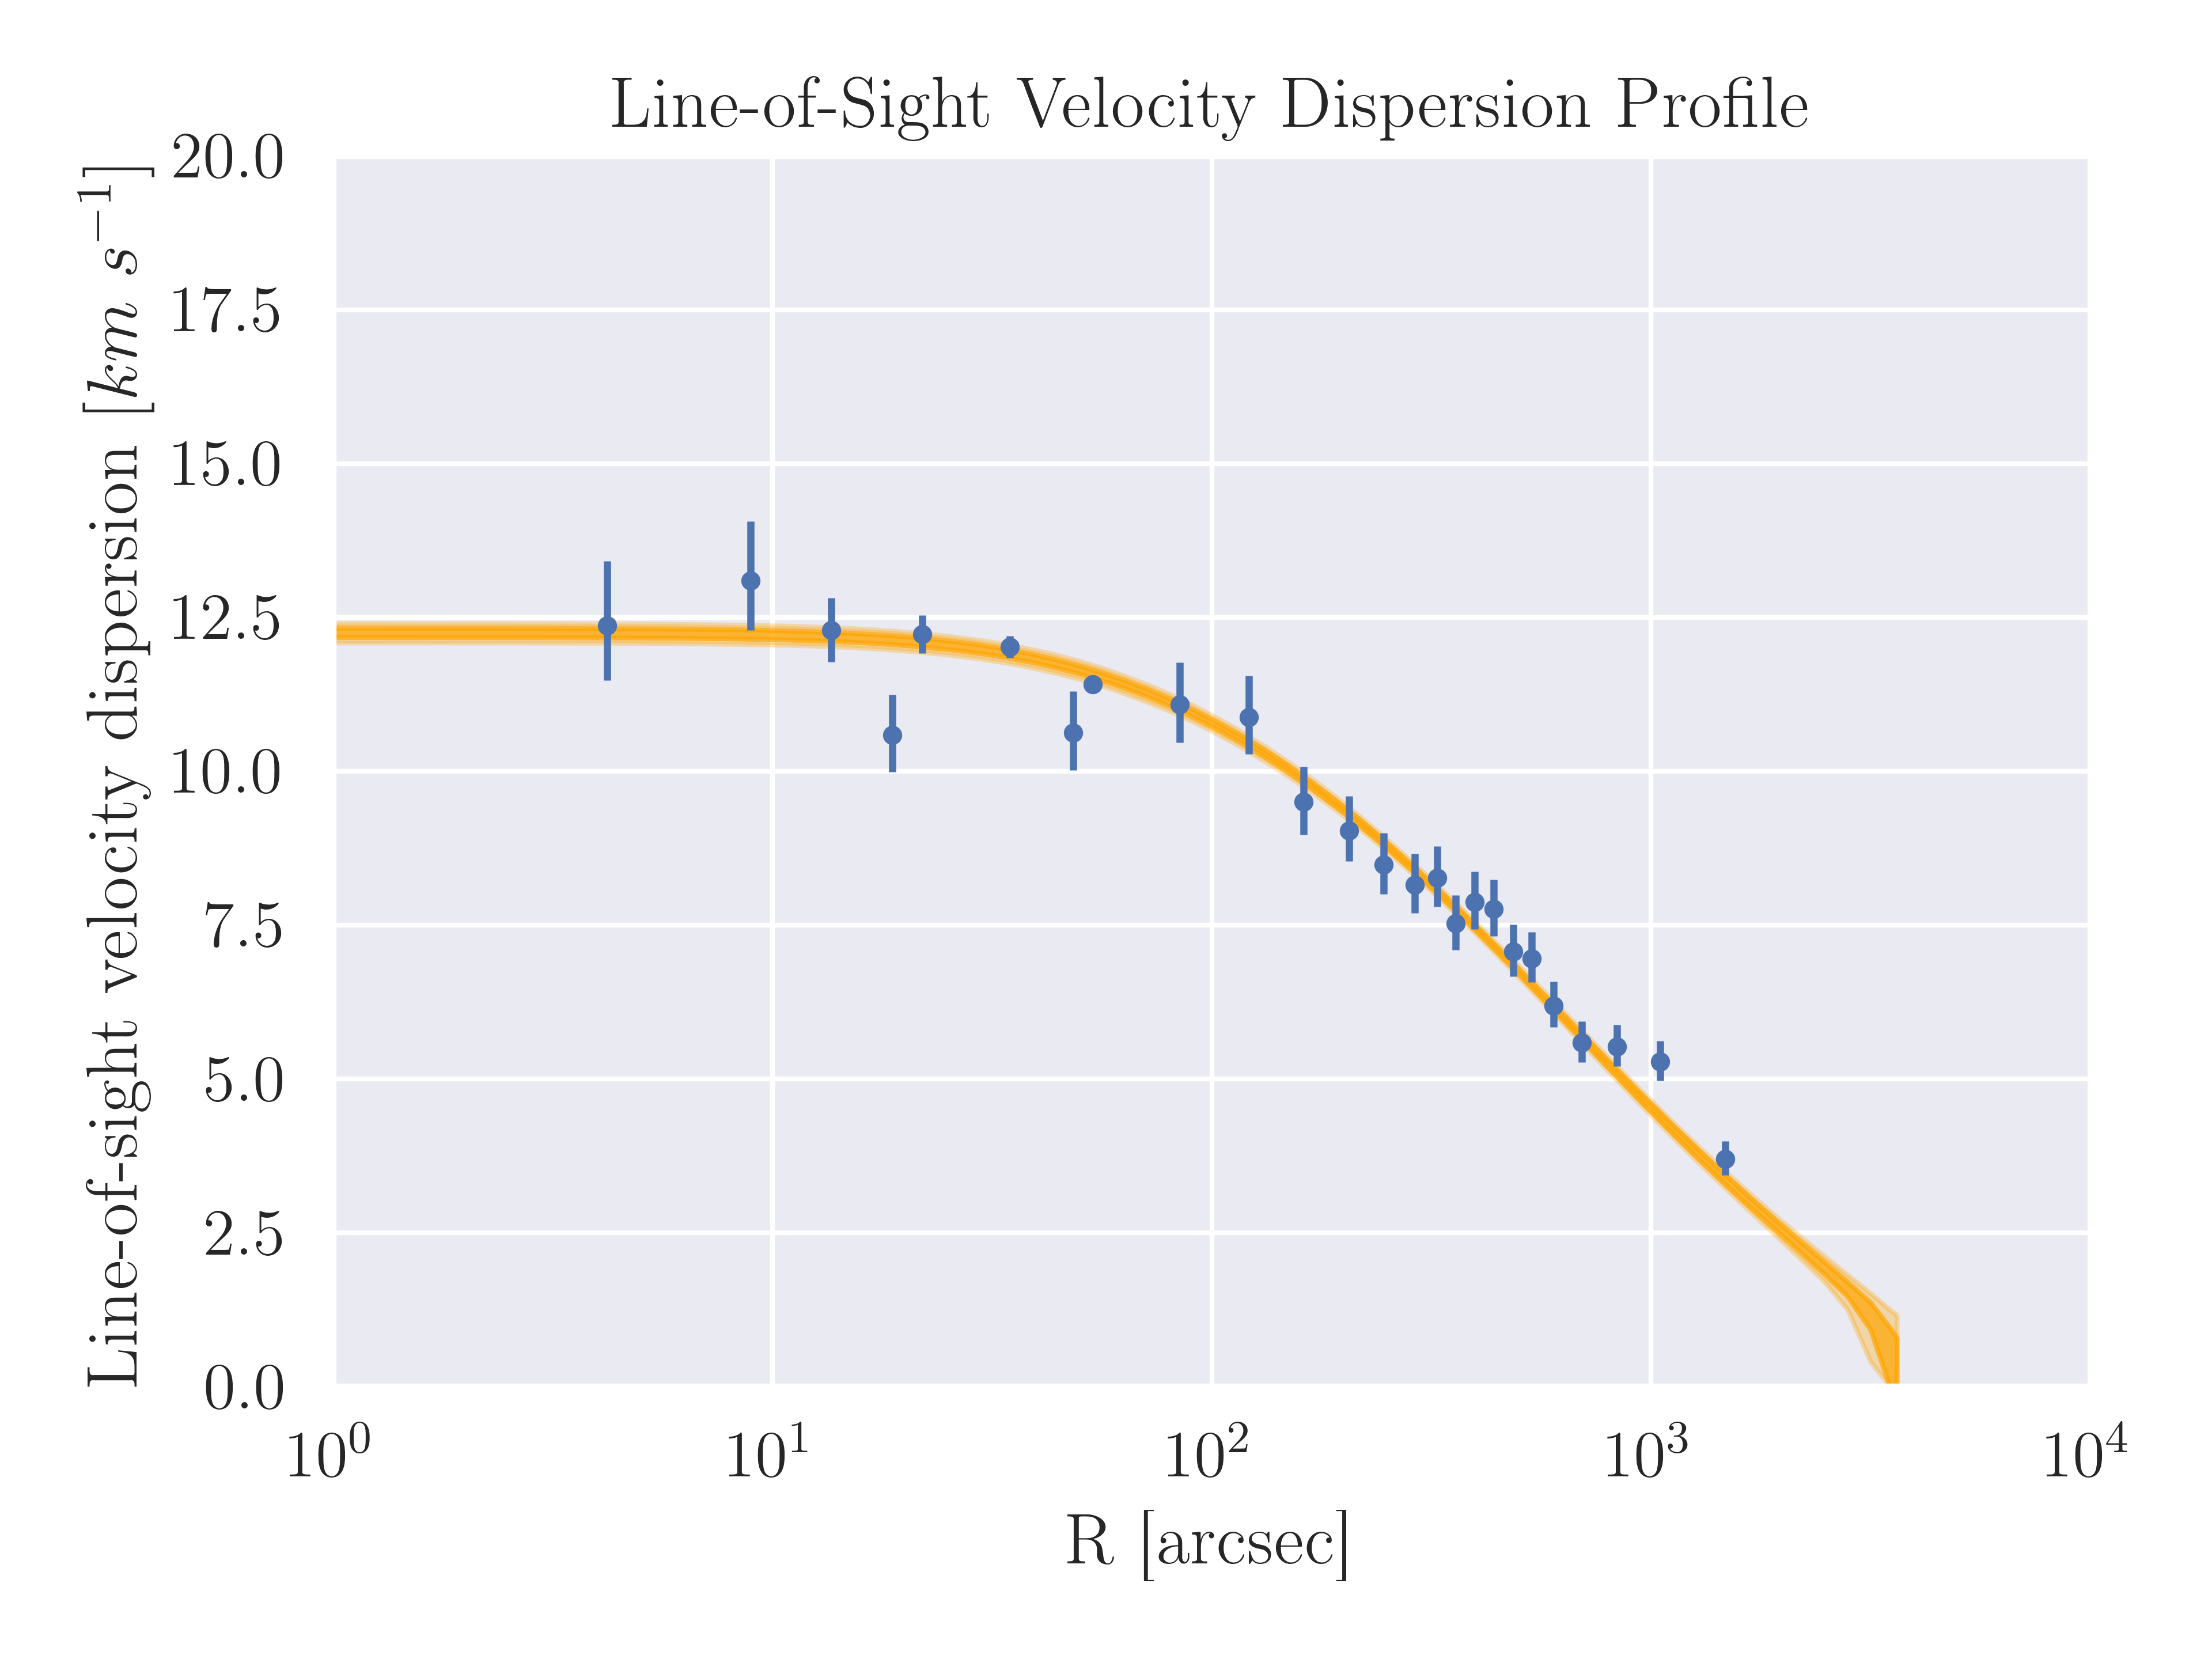
\includegraphics[width=0.8\textwidth]{./figures/limepy_veldisp.png}
	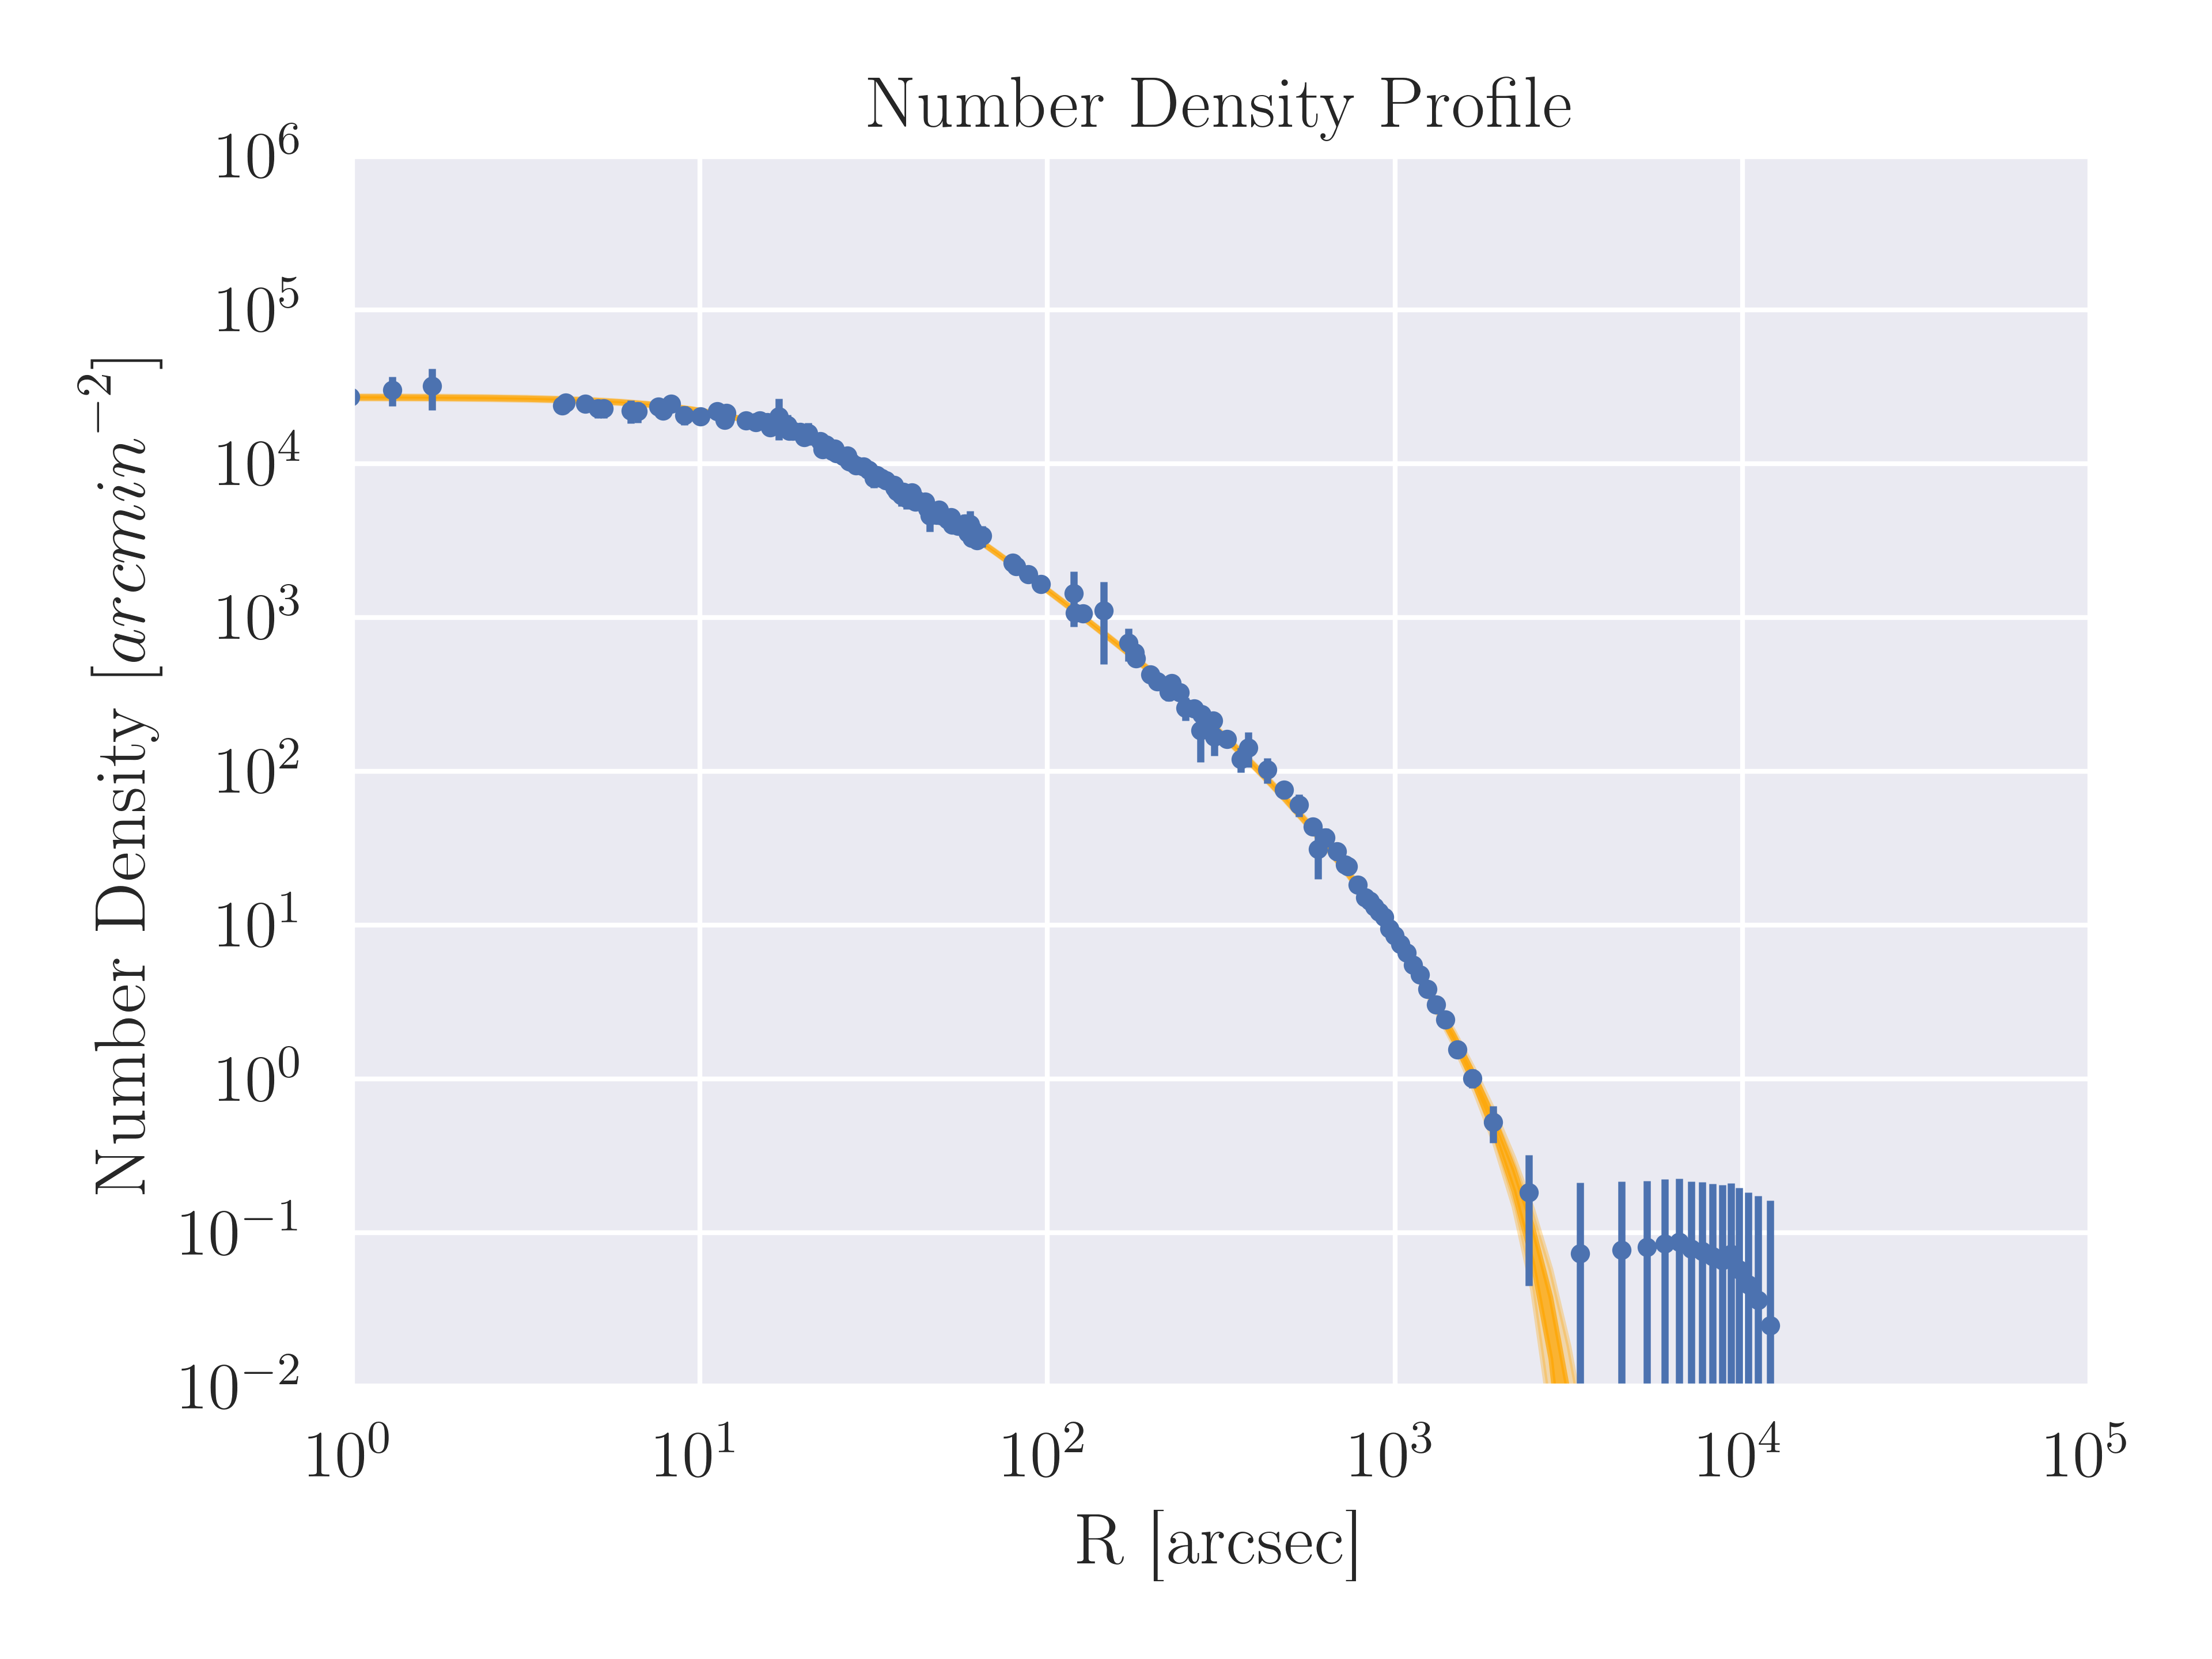
\includegraphics[width=0.8\textwidth]{./figures/limepy_numdens.png}
	\caption{The line-of-sight velocity dispersion profile and number density profile of
		47\,Tuc, simultaneously fit by a \code{LIMEPY} model. The \code{LIMEPY} models are
		able to very accurately reproduce a range of cluster observables including
		simultaneous fitting of stellar mass function data and kinematic data.}
	\label{fig:1/limepy_models}
\end{figure}


The input parameters needed to compute our models include the central concentration parameter $W_0$,
the truncation parameter $g$\footnote{Several well-known classes of models are reproduced by
	specific values of $g$: Woolley models \citep{Woolley1954} have $g=0$, King models \citep{King1966}
	$g=1$, and Wilson models \citep{Wilson1975} $g=2$.}, the anisotropy radius $r_a$ which determines
the degree of radial anisotropy in the models, $\delta$ which sets the mass dependence of the
velocity scale and thus governs the degree of mass segregation, and finally the specific mass bins
to use as defined by the mean stellar mass ($m_j$) and total mass ($M_j$) of each bin, which
together specify the stellar mass function. In order to scale the model units into physical units,
the total mass of the cluster $M$ and a size scale (the half-mass radius of the cluster $r_h$) are
provided as well. Figure \ref{fig:1/limepy_models} demonstrates the ability of the models to
simultaneously fit many cluster observables, specifically pictured are the line-of-sight velocity
dispersion profile and the number density profile, though the power of these models lies in their
ability to simultaneously fit not just kinematic and number density data but also the stellar mass
function data of a cluster.


In their current implementation, these models assume that all objects within the cluster are single
and make no attempt to model the dynamical effects of stellar multiplicity. In this project, we
adapt these models to incorporate some of the effects of binary stars under the assumption that
binaries with very long periods have been ionized by the present day. This allows us to treat binary
systems as point masses and lets us model their dynamics by simply moving some of the mass in stars
into heavier bins according to the specified binary population.



\section{Binary Stars}
\subsection{Binaries in Globular Clusters}


In general, the binary systems found within present-day clusters differ significantly from the field
binaries that are more easily observed. In particular, we expect very few long-period binaries, on
account of them being ionized by the frequent interactions with other cluster members
\citep{Heggie2003}. We frequently use the terms "hard" and "soft" to describe binaries where "soft
binaries" have binding energies less than or comparable to the average kinetic energy of a cluster
member while "hard binaries" have larger binding energies. Due to the frequent interactions within
clusters, we expect that all soft binaries have long since been ionized by the present day leaving
only a population of hard binaries with a truncated period distribution compared to field binaries
\citep{Heggie2003}.




The most obvious way that binaries can affect the dynamics of a cluster is through three- or
four-body interactions with other cluster members. When a single star (or another binary) interacts
with a binary system at a close enough range, if the binary is hard, it will impart some of its
energy to the ejected star and "harden" further. If the binary is soft, it will further "soften",
potentially becoming unbound. Through these processes, soft binaries are slowly disrupted while hard
binaries become harder \citep{Heggie1975}. Hard binary systems can act as a reserve of kinetic
energy for a cluster through these three-body interactions with passing cluster members
\citep{Heggie2003}. Binary stars are thought to be one of the primary mechanisms through which
core-collapse (the collapse of the core of a cluster into extremely high density caused by runaway
mass segregation) is halted in some clusters by continually adding to the energy of stars which
migrate to the central regions, thereby pushing them back out into the extended regions of the
cluster \citep{Chatterjee2013}. Because the models that we will be focusing on do not model the
evolutionary history of individual objects within the cluster, we will instead focus on the second
way that binaries can affect the dynamics of a cluster.

Because binaries are tightly bound, for all interactions except for the very closest, they
effectively act as a single point mass equal to the sum of each component's mass. In this way,
binaries can affect cluster dynamics in much the same way that a large population of heavy remnants
might. Much like black holes and neutron stars, binary systems will migrate to the centre of a
cluster due to the effect of mass segregation. It has been found (e.g. \citealt{Kremer2019}) that a
central population of black holes can fulfill a similar role to binary systems in halting core
collapse by injecting kinetic energy through two-body interactions within the core of the cluster.
This same mechanism could apply with tightly-bound binary systems that have mass-segregated to the
centre of the cluster. This predicted increase in binary fraction as you get closer to the centre of
a cluster is also seen in observations and is illustrated in Figure
\ref{fig:1/radial_binary_fraction} for NGC 3201.

The effect of having a large central population of binaries could be that our models are
overestimating the number of black holes and other high-mass objects (neutron stars, massive white
dwarfs) in the core of the cluster. Because the gravitational potential in the central regions of
the cluster is fairly well constrained by kinematic measurements, if we are missing a significant
contribution from binaries, the models may be compensating for this "missing mass" by adding more
mass to the heavy end of the IMF which would lead to an overestimation of the number of neutron
stars and black holes. By including realistic populations of binary stars in our models, we hope to
recover more accurate remnant populations for present-day clusters.




\begin{figure}
	\centering
	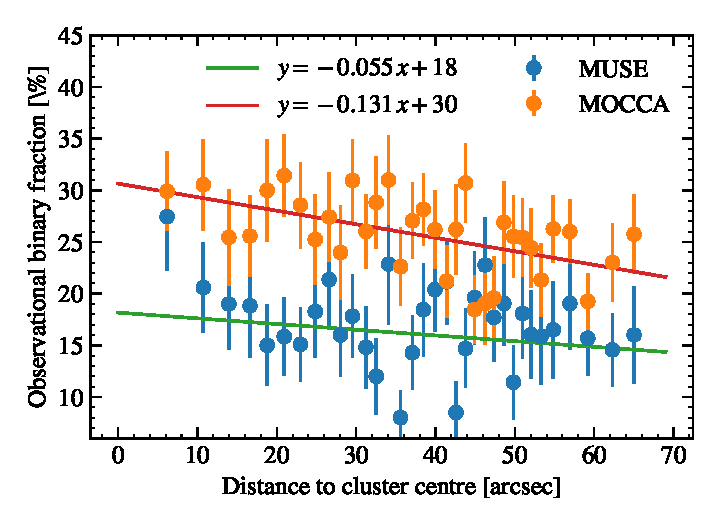
\includegraphics[width=0.8\textwidth]{figures/radial_binarity.pdf}
\caption{Observed binary fraction vs projected distance from cluster centre for NG\,3201 as
	measure by the MUSE instrument. The slight trend in radial binary fraction is
	visible. Also plotted is the observed binary fraction in a MOCCA model which matches
	well with NGC\,3201. MOCCA is a Monte Carlo model designed to model globular
	clusters for which there is a large grid of pre-computed models available.
	Reproduced from Figure 8 of \citet{Giesers2019}.}
	\label{fig:1/radial_binary_fraction}
\end{figure}

\subsection{Observations of Binary Stars in Globular Clusters}

\paragraph{}
In general, there are two methods used to detect binaries within globular clusters: high-precision
photometric observations and radial velocity surveys.

\paragraph{}
High-precision photometry can be used to detect binaries along the main sequence which have a
significant difference in the mass of their components. We often use the ratio between the mass of
the primary star and the companion star to quantify this difference: an equal mass binary will have
a mass ratio of $q=1$ while a binary with a large difference in the masses of its components will
have a mass ratio closer to zero. Binaries that are detectable through this method typically have a
mass ratio greater than $q=0.5$. These systems will appear to be raised above the main sequence when
plotted on a colour-magnitude diagram as their colour will match that of a typical main-sequence
star however their luminosity will be the sum of each component. Figure
\ref{fig:1/main_sequence_binaries} shows the main sequence of the cluster NGC\,2298. The binary
stars in this cluster are visible above the main sequence, raised according to their mass ratio.
\citet{Milone2012} performed high-precision photometry on several globular clusters using the Hubble
Space Telescope's (HST) Advanced Camera for Surveys and were able to place strong constraints on the
binary fraction for binaries with a mass ratio above $q=0.5$. This method allows for large studies
of binary populations in GCs without the need for dedicated observations of individual systems but
suffers from an inherent bias towards systems with high mass ratios. Systems with mass ratios below
$q=0.5$ are typically too close to the regular main-sequence to confidently classify as binaries
(see Figure \ref{fig:1/main_sequence_binaries}). This means that studies that employ this method
must assume an underlying mass-ratio distribution for low values of $q$ if they wish to place any
limits on the overall binary fraction of a cluster. Typical values for the binary fraction in
massive clusters found using this method range from almost zero to an upper limit of around $15\%$
\citep{Milone2012}. Additionally, studies of the mass ratio distribution within these clusters using
the same method find a preference for a uniform or "flat" distribution unlike the distribution in
the solar neighbourhood which is peaked at $q=1.0$ \citep{Milone2012,Fisher2005}


\begin{figure}
	\centering
	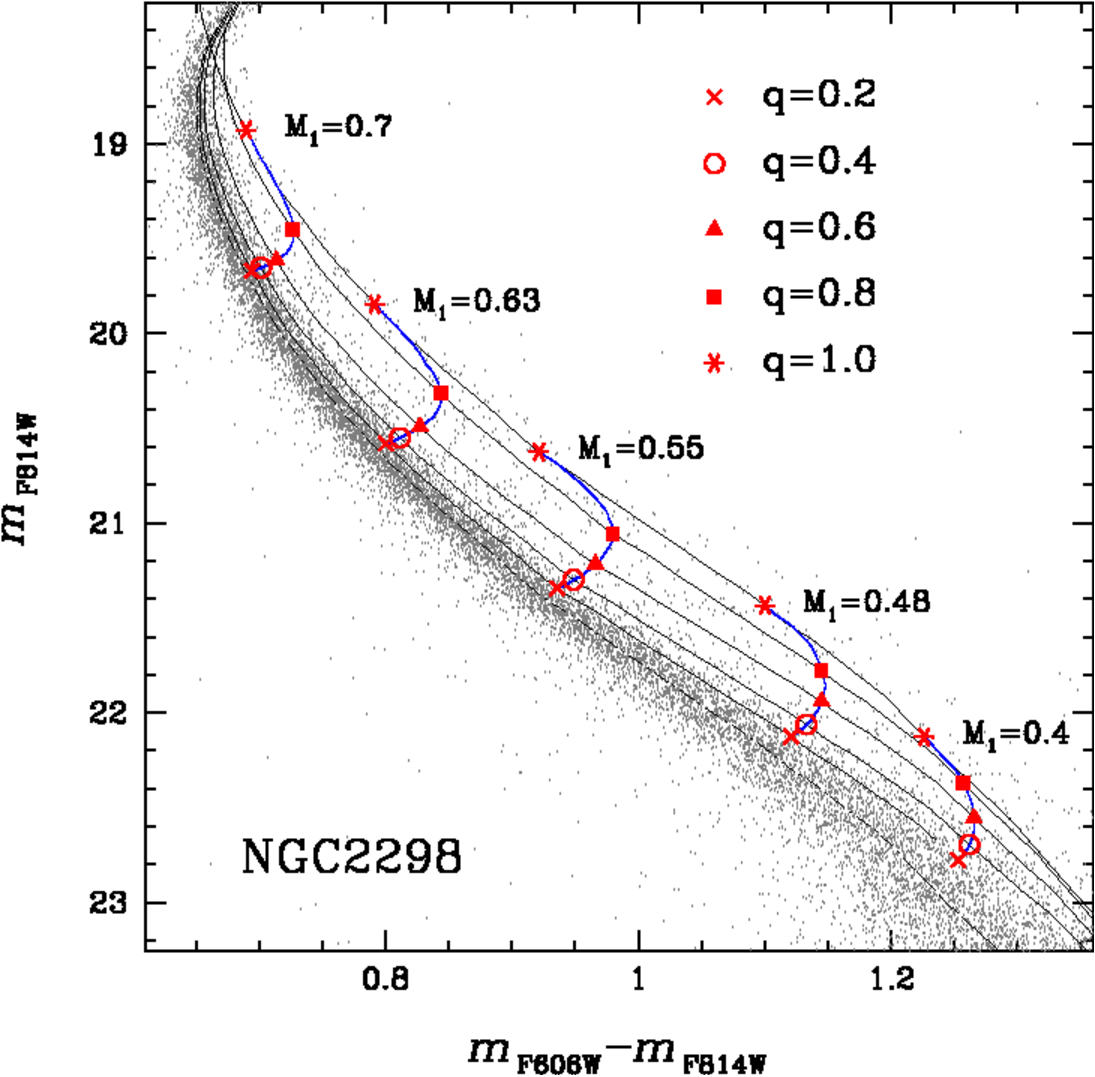
\includegraphics[width=0.8\textwidth]{./figures/main_sequence_binaries.pdf}
	\caption{The main-sequence portion of the colour-magnitude diagram for NGC\,2298. Binary
systems are visible as being raised above the primary main sequence with systems
with a higher mass ratio being raised further off of the main sequence. Systems
below a mass ratio of $q=0.5$ are nearly indistinguishable from the regular spread
in main sequence stars. Reproduced from Figure 1 of \citet{Milone2012}.}
	\label{fig:1/main_sequence_binaries}
\end{figure}

\paragraph{}
Large-scale campaigns to measure the radial velocities for many stars in a cluster over many epochs
are another method that can be used to detect binaries in GCs. Systems that are found to have
periodically varying radial velocities can typically be confidently classified as binary systems.
\citet{Giesers2019} used the MUSE integral field spectrograph installed at the European Southern
Observatory's Very Large Telescope to observe several GCs and reported the results for NGC\,3201.
Integral field spectrographs provide spatially resolved spectra for the entire field of view of the
detector which enables far more time-efficient surveys than previous methods. Because this method
measures radial velocities over time, periods for the binaries can be accurately determined and
given enough measurements, many other parameters like eccentricity and companion mass can be
accurately constrained in contrast to photometric methods which can only provide the mass ratio.
This method also suffers from biases in that it requires the primary star of a binary to be bright
enough to enable good spectroscopic measurements which may bias the sample towards systems with more
massive primary stars. For NGC\,3201, the binary fraction found using this method was $6.75 \pm 0.72
	\%$ \citep{Giesers2019} which differs from the photometric estimates of \citet{Milone2012} which
range from $10\textrm{-}12\%$ for different fields.


\paragraph{}
The remainder of the thesis is structured as follows: in Chapter 2 I will describe the method used
to generate mass functions which include realistic binary populations as well as the specifics of
fitting these modified mass functions to real observations of stellar mass functions. Chapter 3
discusses the results of the simulations, including the differences between models with and without
binaries. Chapter 4 discusses the overall implications of including binaries in our models,
specifically when fitting them to observations.



